\documentclass{article}
\usepackage{amsfonts}
\usepackage{graphicx}
\usepackage[margin=1in]{geometry}
\usepackage{bm}
\usepackage{amsmath}
\usepackage{authblk}
\usepackage{caption}
\usepackage{hyperref}
\usepackage{float}
\usepackage[parfill]{parskip}
\newcommand{\overbar}[1]{\mkern 2mu\overline{\mkern-2mu#1\mkern-20mu}\mkern 20mu}

\title{Supplementary Materials for cILR: Taxonomic enrichment analysis with isometric log ratios}
\begin{document}
\author{Quang P. Nguyen, Anne G. Hoen, H. Robert Frost}
\maketitle
\captionsetup[figure]{labelfont={bf},name={Figure},labelsep=period, margin=1cm}


\section{Addressing variance inflation due to correlation}
In order to perform inference with competitive isometric log ratio (cILR), we estimated the null distribution empirically following Efron et al. \cite{efron2004}. We chose two distributional forms for the null: the normal distribution and a two-component mixture normal distribution. Subsequently, we estimated the parameters of the respective distributions from a column (or variable) permuted raw score matrix. This means that our null distribution for a given set is equivalent to scores computed for sets of similar sizes but containing randomly chosen taxa. For the normal distribution, we estimated parameters using the maximum likelihood using the \emph{fitdistrplus} package \cite{delignette-muller2015}. For the mixture normal distribution, we utilized the expectation-maximization procedure from the package \emph{mixtools} \cite{benaglia2009}. 

However, when variables are correlated, the variance of the sample mean of the variables is inflated \cite{wu2012}. Without loss of generalizability, for a set of variables $x_1, ..., x_p$ we have the variance of the mean $\bar{x}$ to be:  
\begin{equation} \label{eq:1}
    Var(\bar{x}) = \frac{1}{m^2}\left(\sum_{i = 1}(\sigma_i^2) + \sum_{i < j}\rho_{ij}\sigma_i\sigma_j\right)
\end{equation}
where $\sigma_i$ is the standard deviation of variable $i$ while $\rho_{ij}$ is the correlation between $i$ and $j$. The second term of (\ref{eq:1}) is the correlation dependent variance component, which goes to 0 if there is no correlation. Wu et al. \cite{wu2012} showed that a null distribution estimated from a column permuted matrix does not account for this variance inflation, since the permutation procedure disrupts the natural correlation structure of the original variables. 

The cILR statistic follows a similar pattern. Since the geometric mean of a set of variables is equivalent to the exponential of the arithmetic mean of their logarithms, we can re-write cILR for a set $k$ with size $\kappa$ as follows:  
\begin{equation}\label{eq:2}
    cILR_k = \sqrt{\frac{\kappa(p - \kappa)}{\kappa + (p - \kappa)}} \left( \overbar{\log{X_{j|j \in K}}} - \overbar{\log{X_{j|j \notin K}}} \right)   
\end{equation}
where $p$ is the overall number of taxa, $j$ is the index of a taxa and $K$ is the set of indices of taxa in set $k$. The cILR statistic then looks similar to a t-statistic for difference in means of log-transformed proportions. As such, the pooled variance of cILR is dependent on the variance inflation of both mean components $\overbar{\log{X_{j|j \in K}}}$ and $\overbar{\log{X_{j|j \notin K}}}$. 

It is important to address this problem since there is strong inter-taxa correlation within the microbiome \cite{kurtz2015}. Even though Wu et al. proposed a correlation adjusted t-statistic for the CAMERA method \cite{wu2012}, it is difficult to adapt such modifications to the cILR statistic. This is because CAMERA requires an estimation procedure for pair-wise correlations of the $\log{X_j}$, as well as making the assumption that the marginal variance of each $\log{X_j}$ is equivalent to each other. 

Instead, our strategy is to combine the location (or mean) estimate from the column permuted raw score matrix with the spread (or variance) estimate from the original un-permuted scores. This still allows us to leverage the null generated via column permutation while using the proper variance estimate taken from scores where the correlation structure has not been disrupted. As such, this procedure assumes that the variance of the test statistic under the alternate hypothesis is the same as that of the null.  

For the normal distribution, it is straightforward to combine mean and variance estimates from the respective raw score matrices. For the mixture normal distribution, however, due to the fact that the distribution is made of component-wise means, variances and mixing coefficients, we decided to take an optimization based approach to identifying the component wise variances $\sigma_1$ and $\sigma_2$ such the overall mean and variance estimates come from the respective raw cILR score matrices as detailed above. We can write the optimization problem as follows: 

\begin{equation} \label{eq:3}
\begin{aligned}
    \min_{\sigma_1, \sigma_2} \quad & \sqrt{\left(\sqrt{(\sigma_1 + \mu'_1 - M')\lambda'_1 + (\sigma_2 + \mu'_2 - M')\lambda'_2} - SD\right)^2}\\
    \textrm{s.t.}  \quad & \sigma_1 \geq 10^{-5}, \sigma_2 \geq 10^{-5}    \\
    \textrm{where} \quad & M', SD, \mu'_1, \mu'_2, \lambda'_1, \lambda'_2 \text{ are constants} \\
\end{aligned}
\end{equation}
$\lambda'_1$, $\lambda'_2$, $\mu'_1$, $\mu'_2$, and $M'$ are component-wise mixing coefficients, component-wise means, and overall mean of the mixture distribution estimated from column-permuted scores while $SD$ is the overall standard deviation of the mixture distribution estimated from unpermuted scores. We solve for this optimization problem using a quasi Newton method with box constraints (L-BFGS-B) with the default finite-difference approximation of the gradient, as implemented in the \emph{optim} function in R.   

\section{Performance evaluation} 
We implemented cILR in the package \emph{teaR} on GitHub with \emph{Rcpp} implementations for geometric mean computations. We evaluated computational time using the \emph{bench} package in R. Sample size and number of sets were varied across different evaluation conditions. All set sizes were kept constant at 50. 

\begin{figure}[!ht]
    \centering
    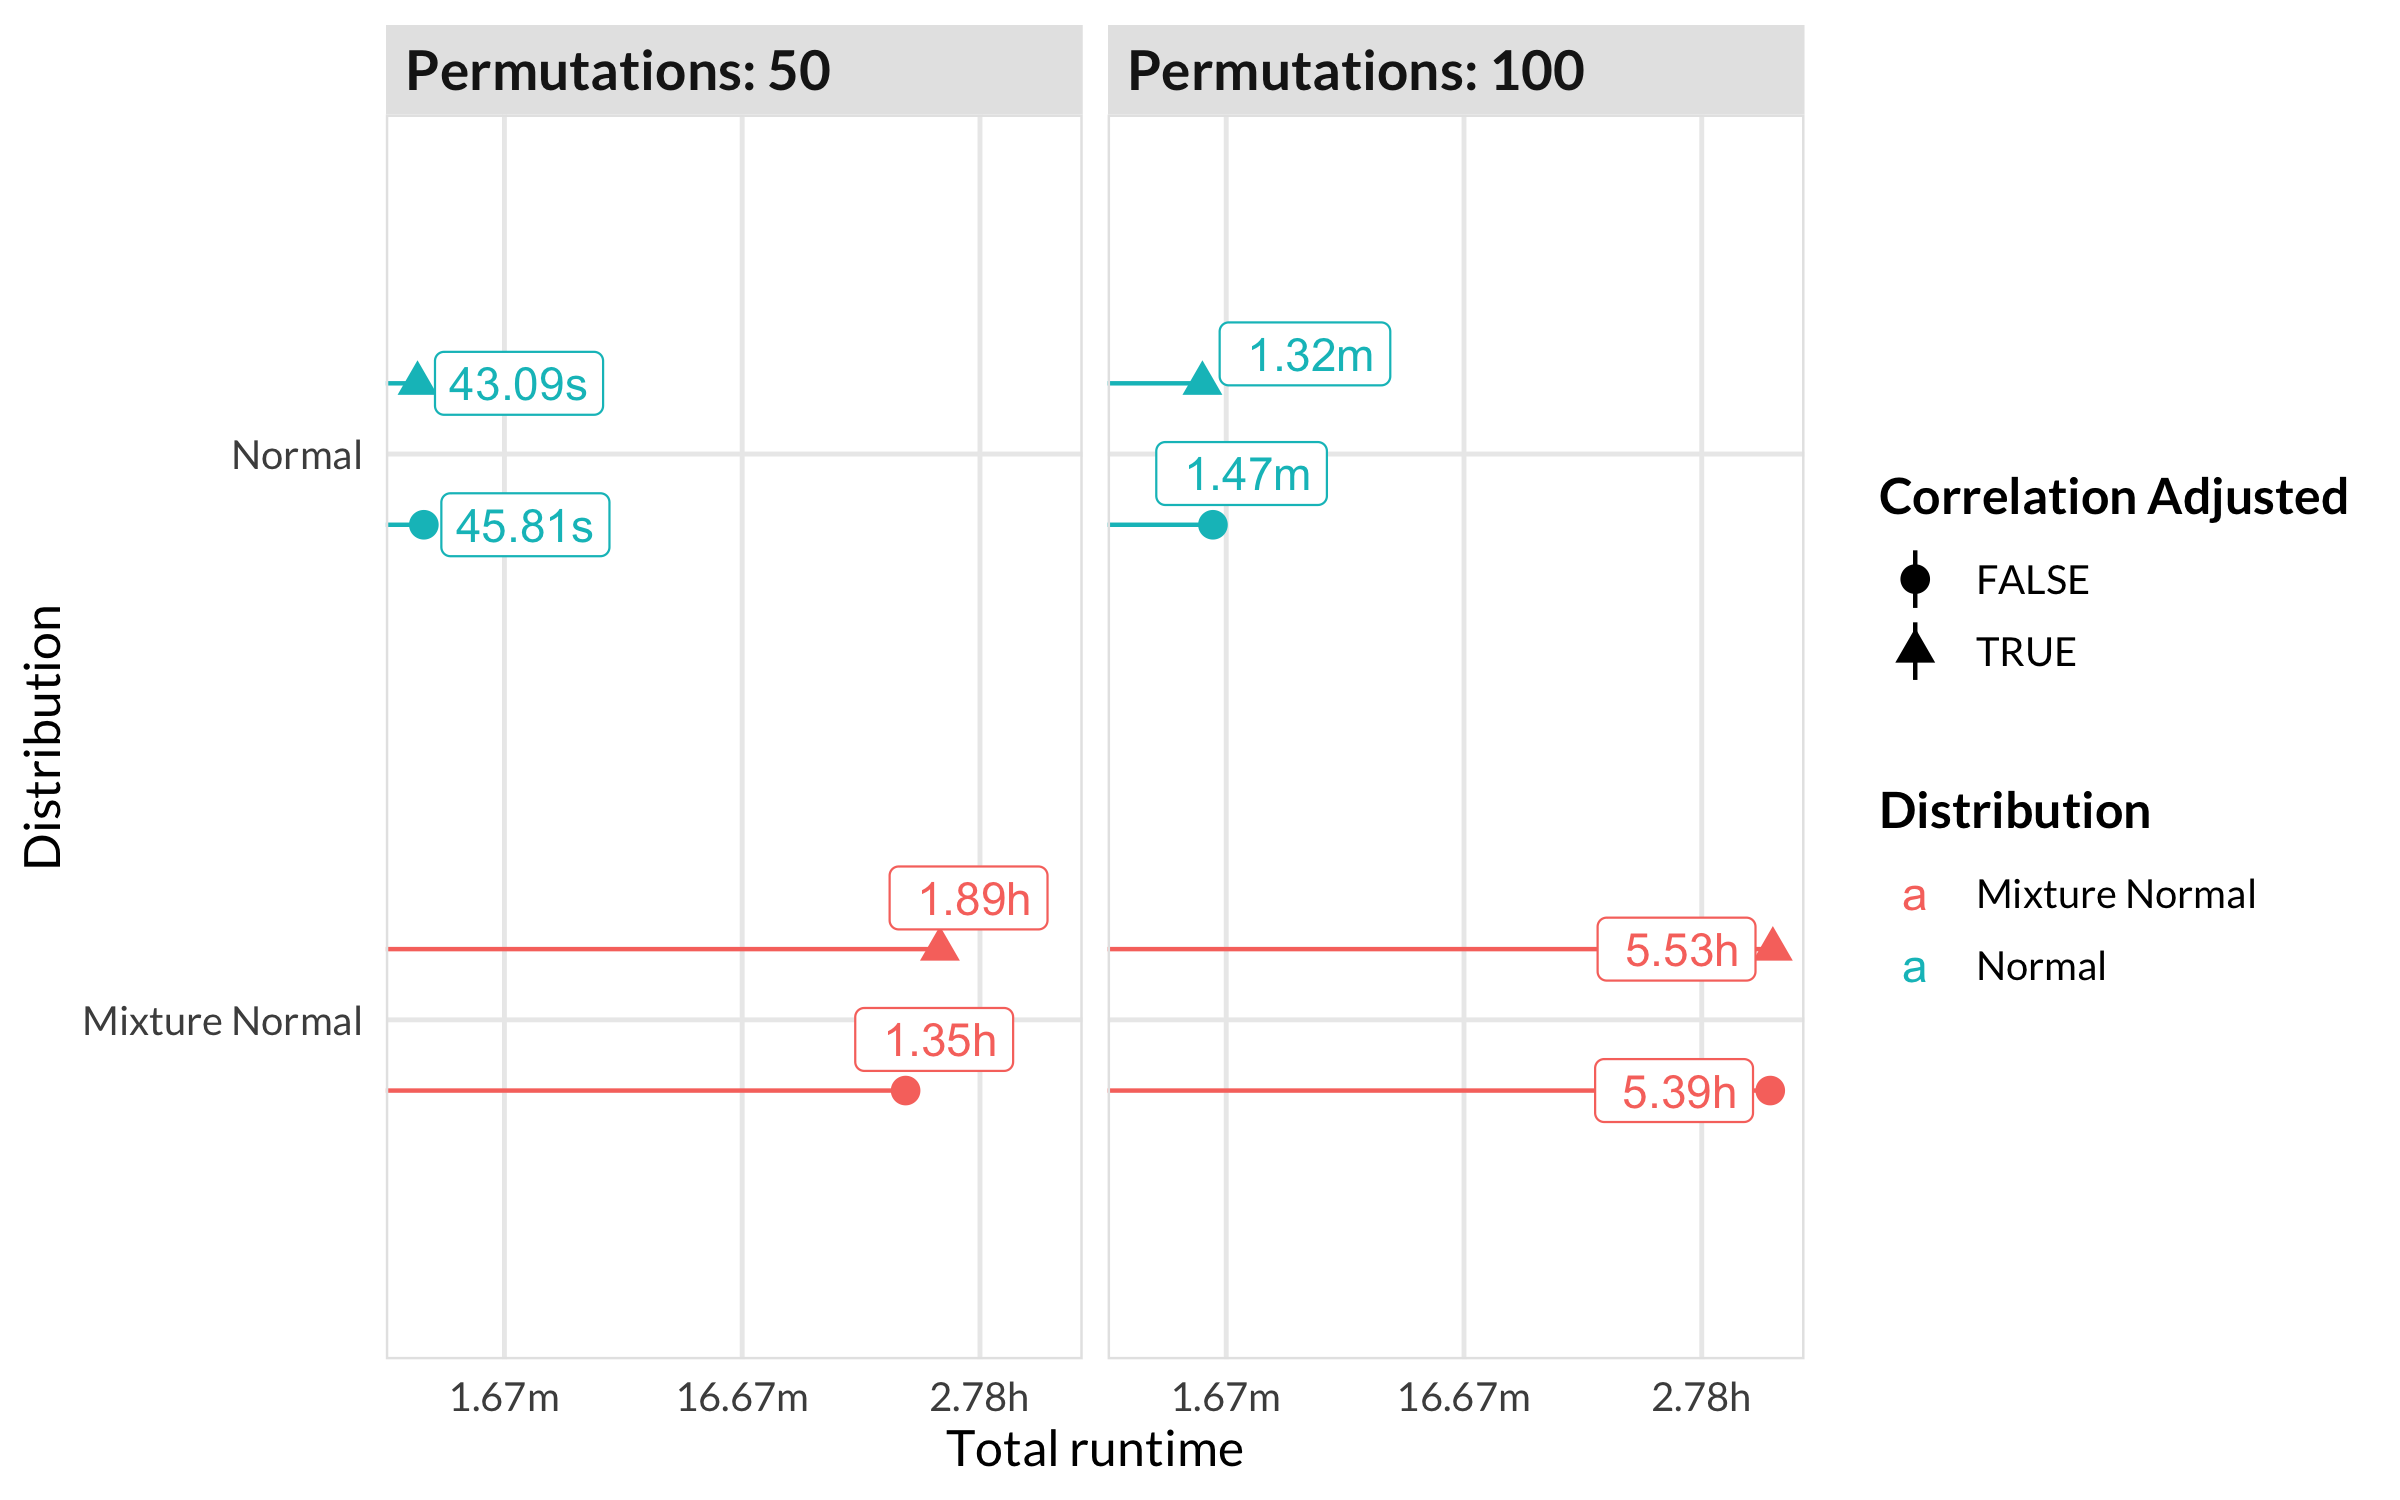
\includegraphics[width=\textwidth]{figures/performance.png}
    \caption{Computational time (in seconds) as a function of sample size (left panel) and number of taxa sets evaluated (right panel). Evaluation was performed on simulated data sets. For sample size analysis, only 10 sets were evaluated. For taxa set analysis, sample size was fixed at 1,000. Across all evaluations, the size of each taxa set was also fixed at 50.}
    \label{fig:s1}
\end{figure}

In general, increasing sample size and number of evaluated sets both increase computational time. The mixture normal distribution takes longer to compute compared to the normal distribution, and adjusted methods take longer but was most apparent when combined with the mixture distribution. Overall, a reasonable data set of 1,000 samples and 100 sets (5,000 taxa) would take around 200 seconds (or approximately 3 minutes) for the longest approach (correlation adjusted mixture normal distribution). Benchmark was performed on a single core using a personal Windows laptop (Specifications: Intel Core i7-9750H (2.6-4.5 GHz - 12MB Cache) with 16GB of RAM)

\section{Distribution of p-values}
We also demonstrate the validity our inference procedure by assessing the distribution of p-values. We used simulated data sets as described in the main manuscript, under different data sparsity levels (0, 0.6) and inter-taxa correlation within the set ($\rho$ = 0, 0.5). We evaluated p-values of the correlation adjusted method for $\rho = 0.5$ case and the p-values of the unadjusted method for $\rho = 0$ case.  

In general, sparsity has no effect on the distribution of p-values, where it remains uniform at zero correlation values. However, for higher correlation values, p-values deviate more from uniform under the global null, with the mixture normal distribution being further away from uniform compared to the normal distribution. 

\begin{figure}[!ht]
    \centering
    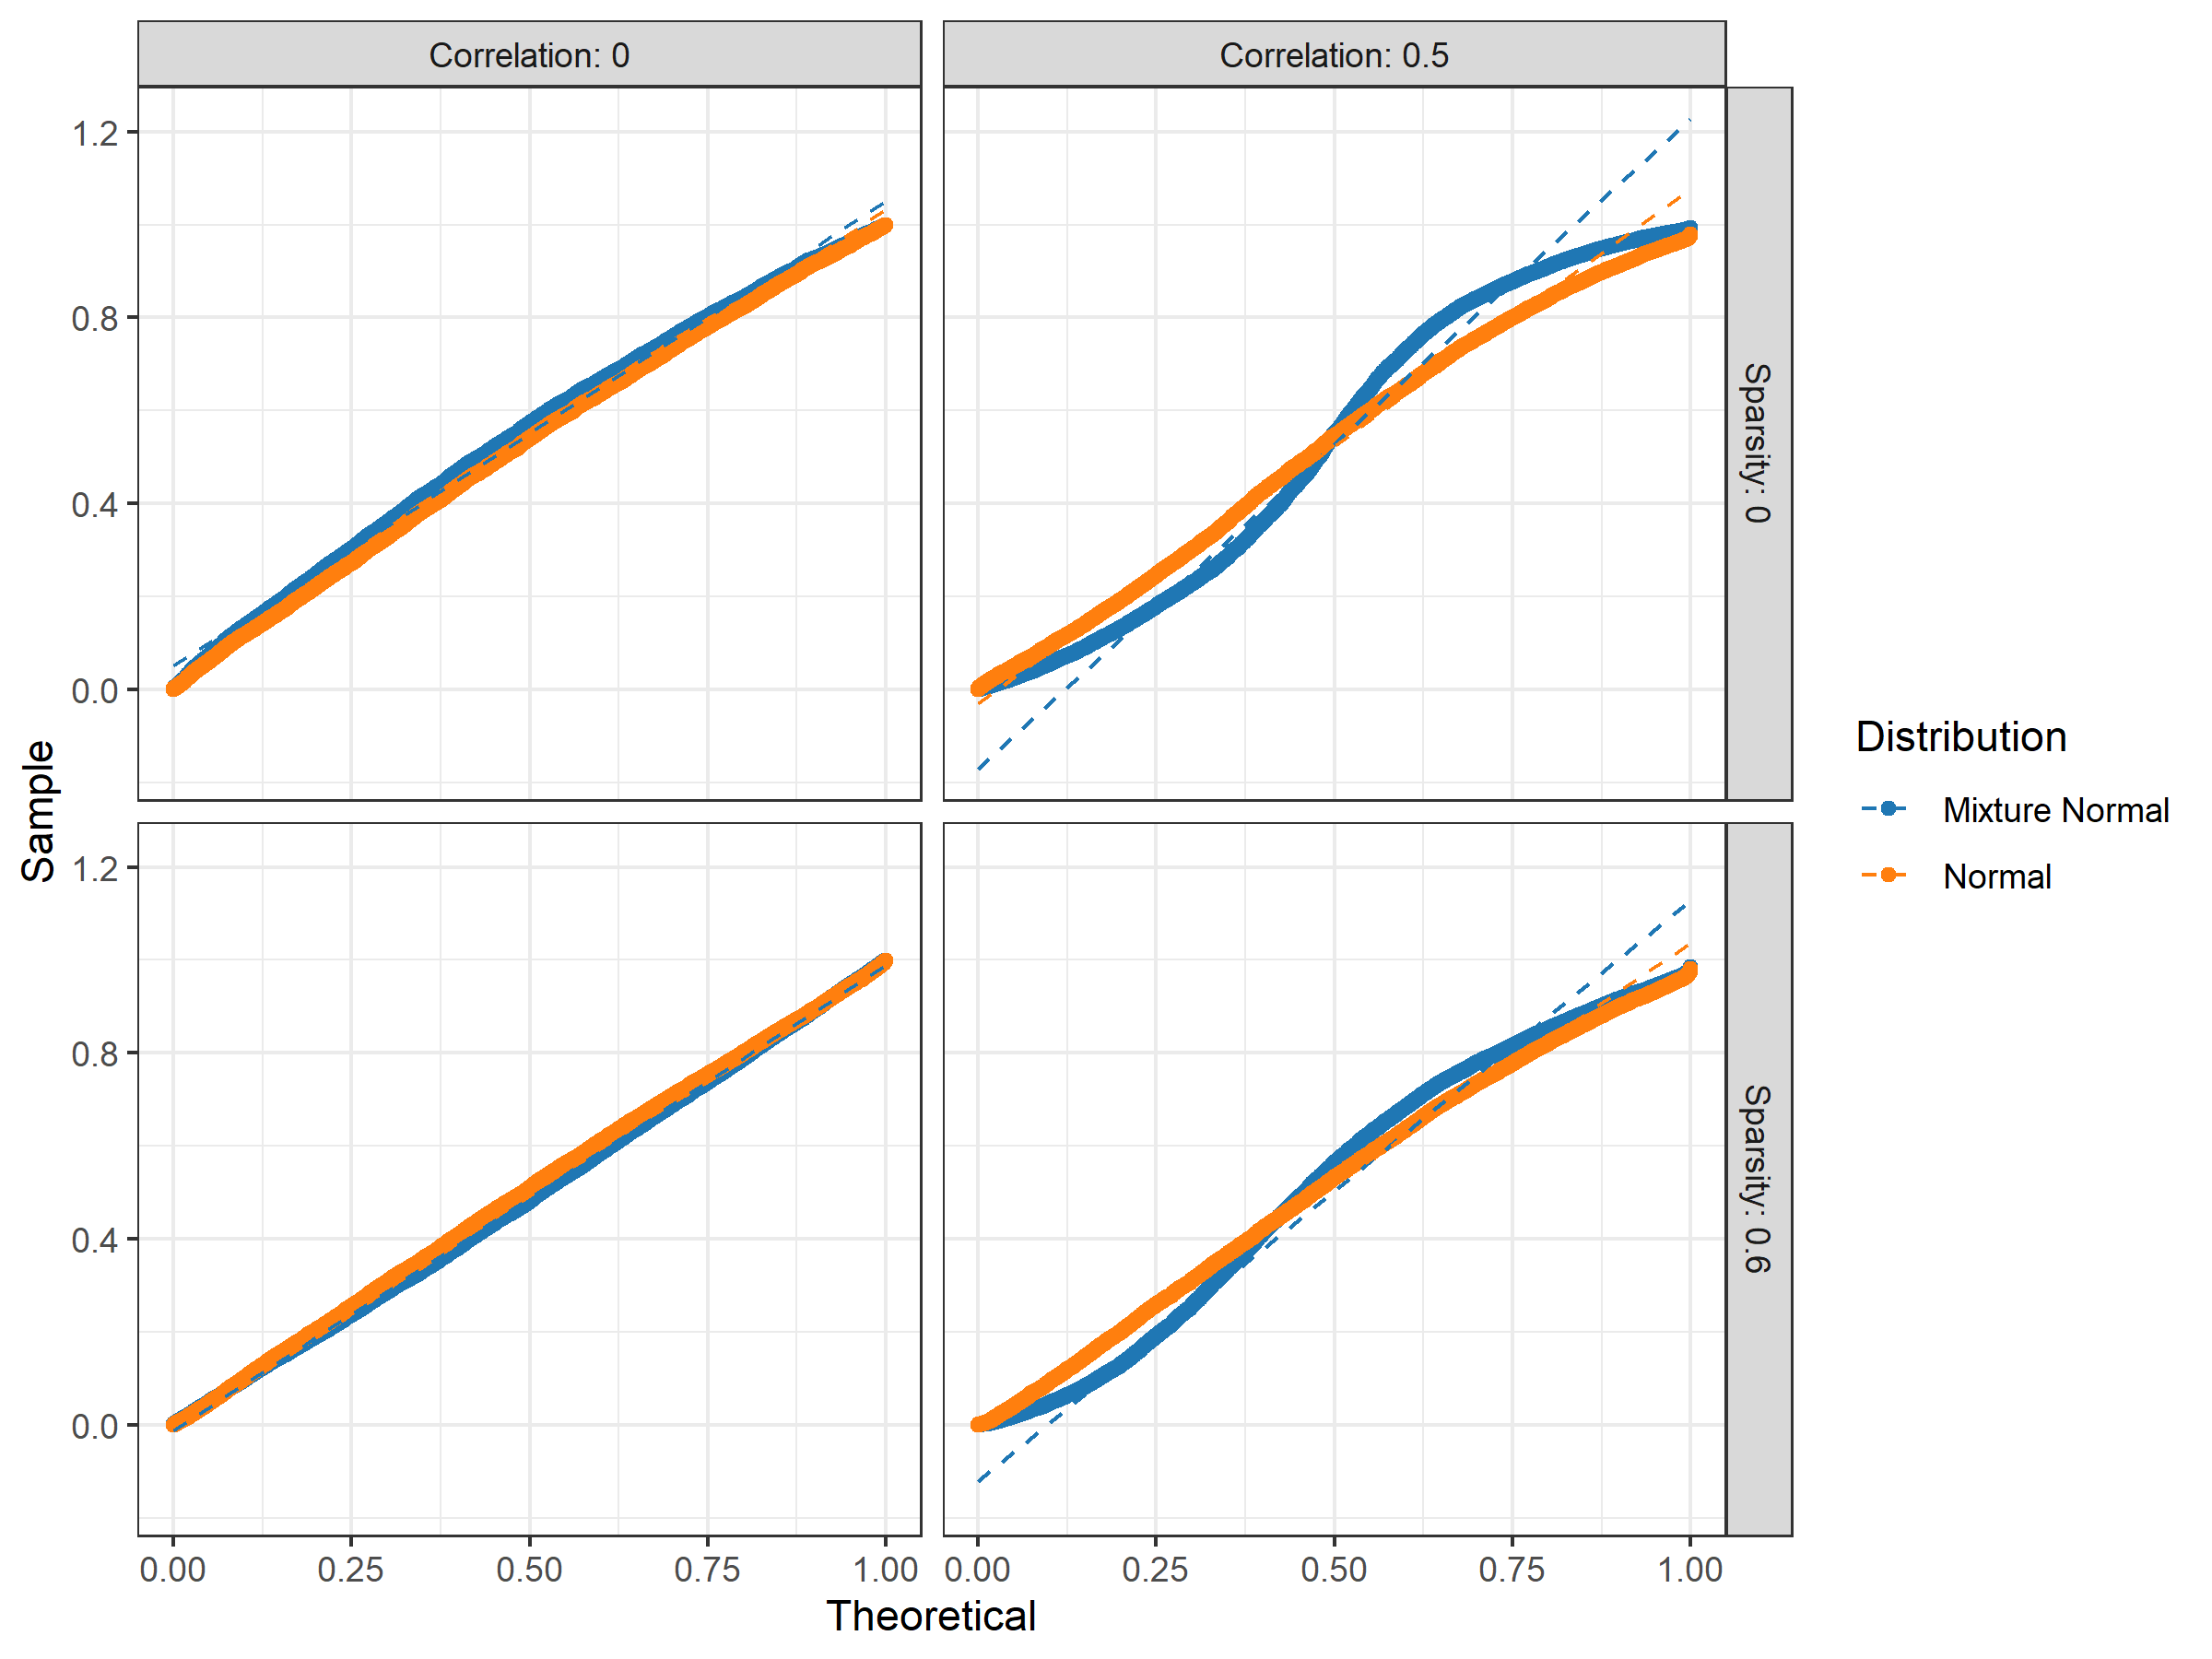
\includegraphics[width=\textwidth]{figures/pval_distr.png}
    \caption{Q-Q plot of 10,000 p-values compared against a uniform distribution bounded between 0 and 1. Evaluation was performed on simulated null data sets of 10,000 samples testing for enrichment of a set of size 50. For correlation of 0.5, p-values represent correlation adjusted cILR while for correlation of 0, p-values represent unadjusted cILR.}
    \label{fig:s2}
\end{figure}

\newpage
\bibliography{tax_agg}{}
\bibliographystyle{plos2015}

\end{document}